\section{Amplitudes at the remaining momenta}
\label{app:amps}
\begin{figure*}[htbp]
\centering
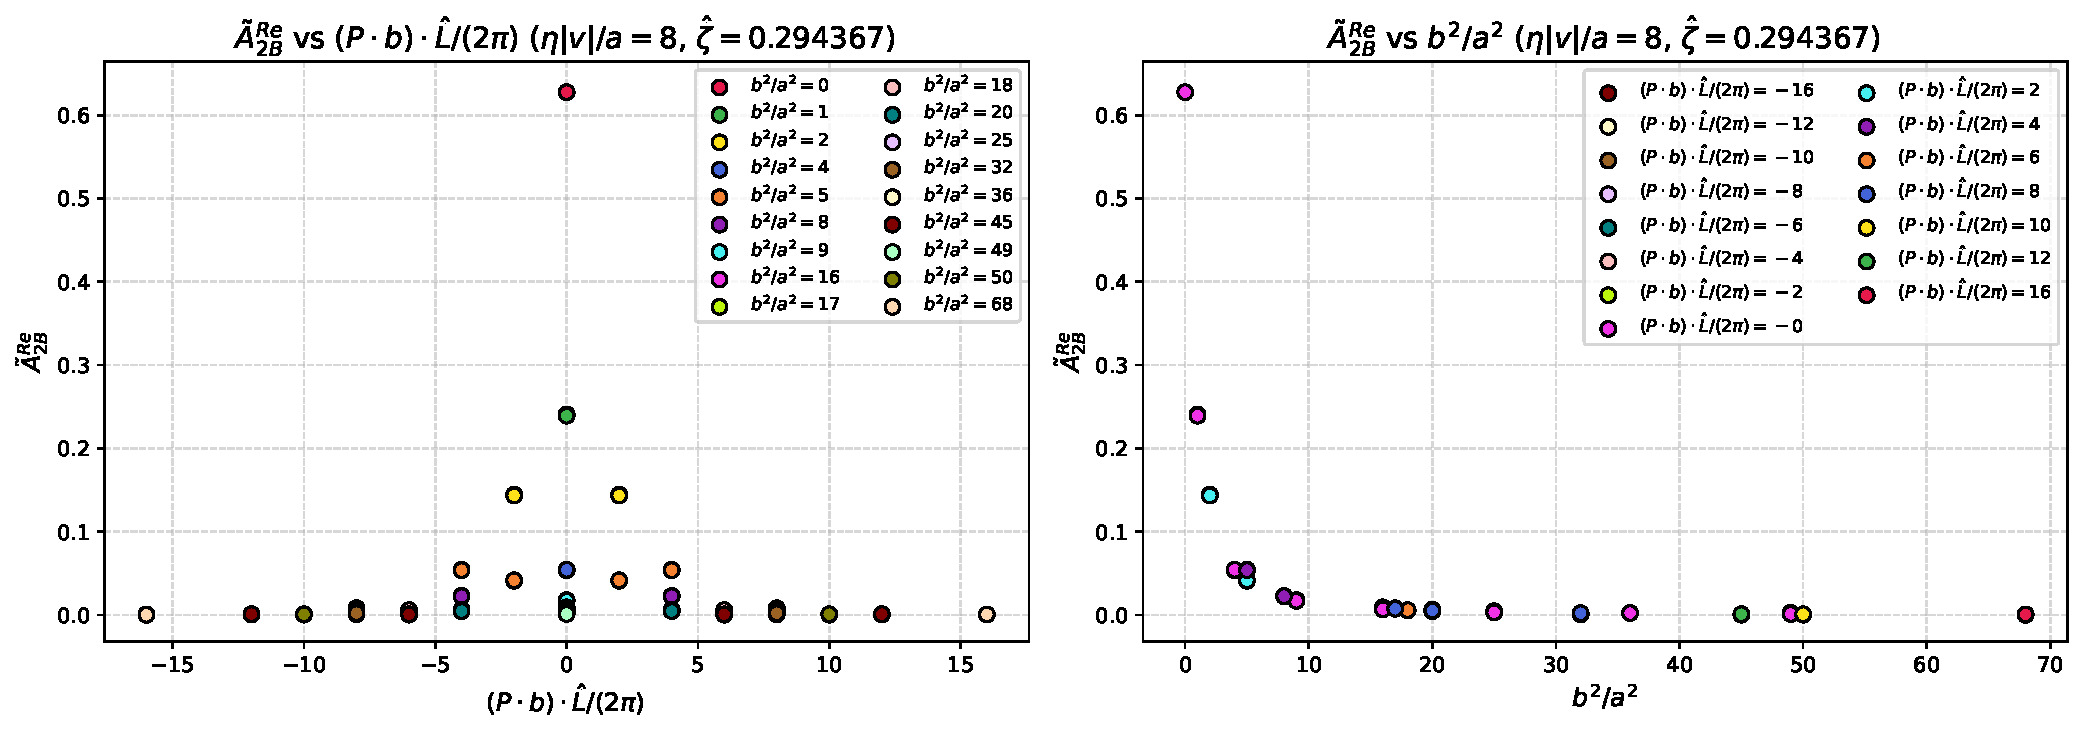
\includegraphics[width=0.48\linewidth]{figures/amps/ReA2B_Pb_bsq_eta8_PL-2_2D.pdf}\hfill
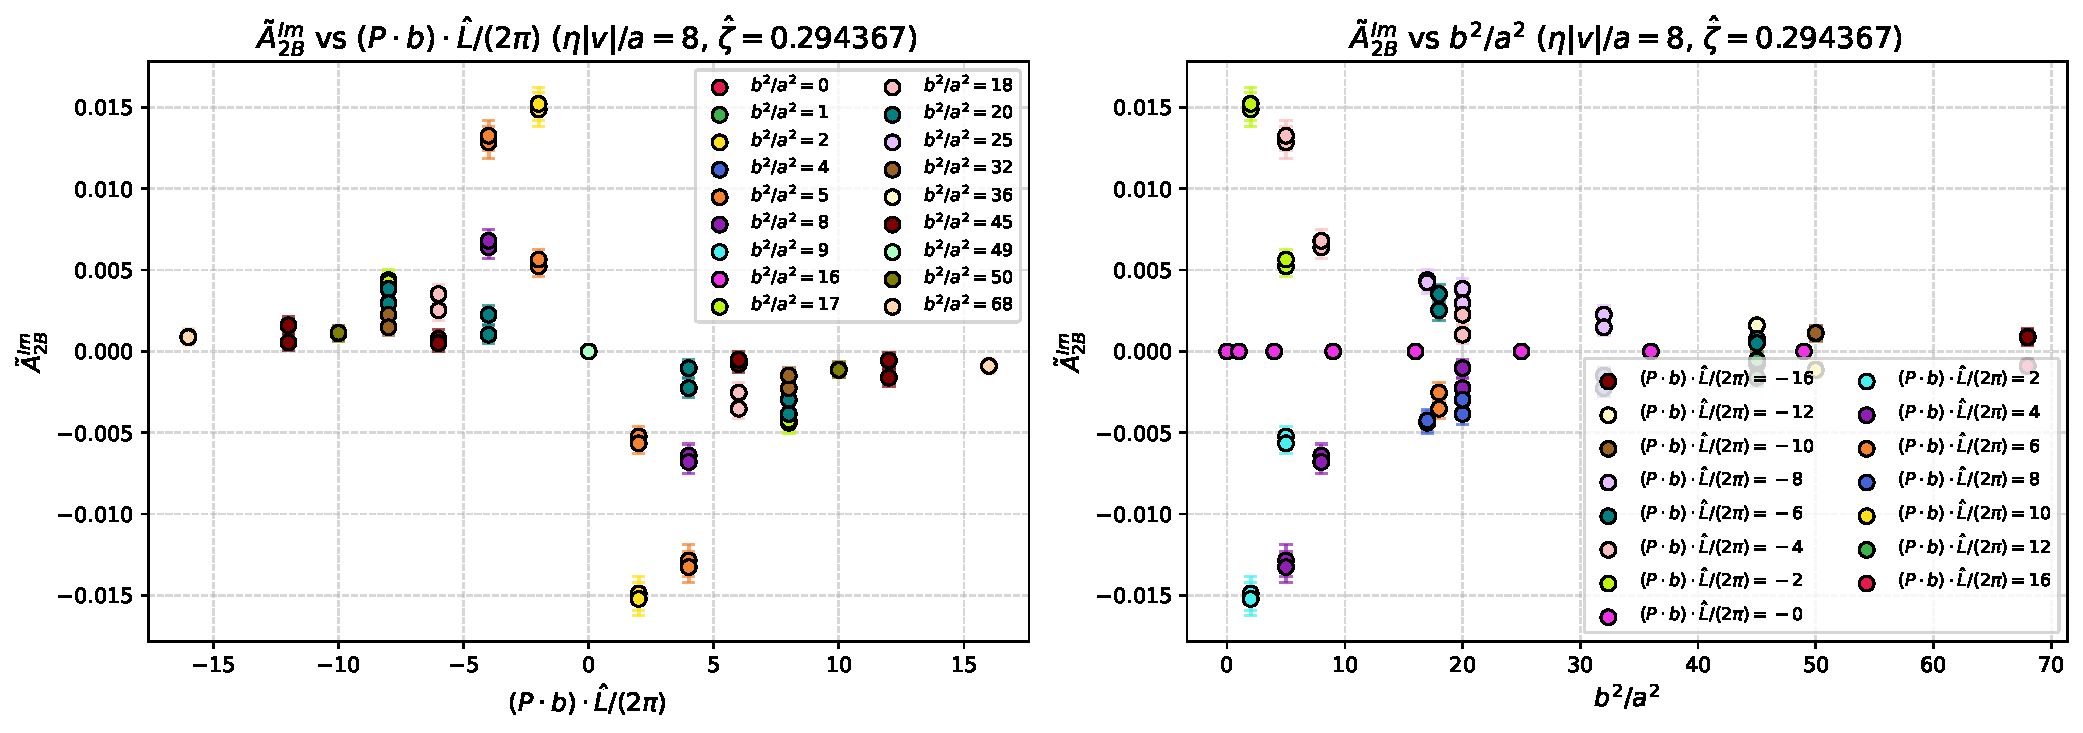
\includegraphics[width=0.48\linewidth]{figures/amps/ImA2B_Pb_bsq_eta8_PL-2_2D.pdf}\\[1ex]
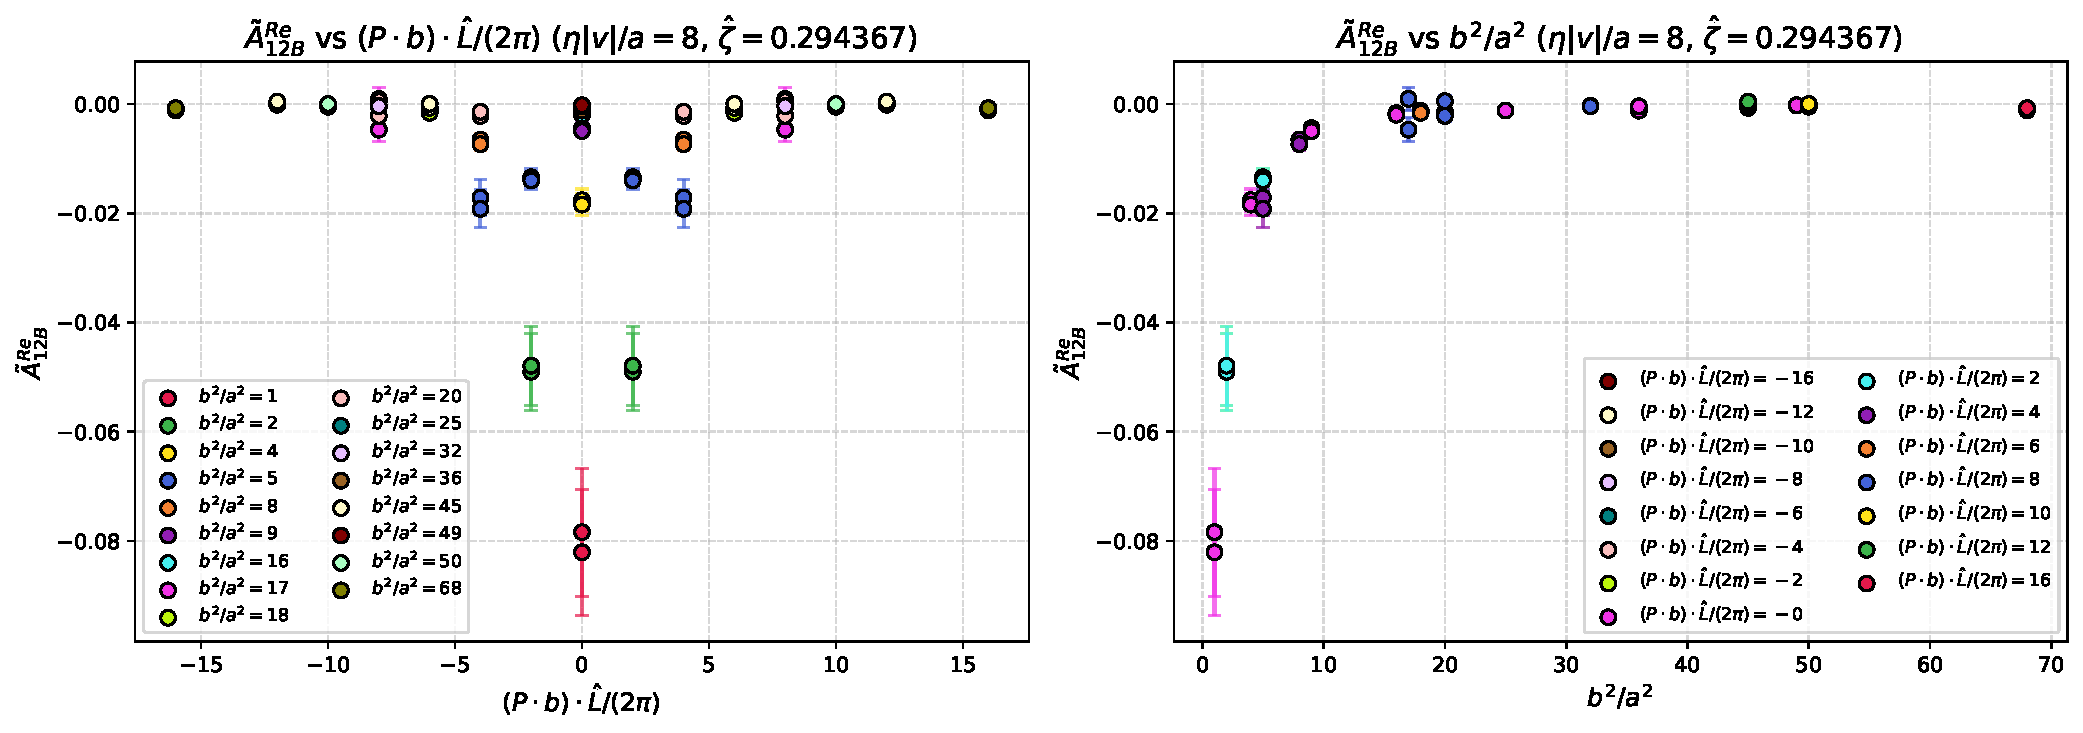
\includegraphics[width=0.48\linewidth]{figures/amps/ReA12B_Pb_bsq_eta8_PL-2_2D.pdf}\hfill
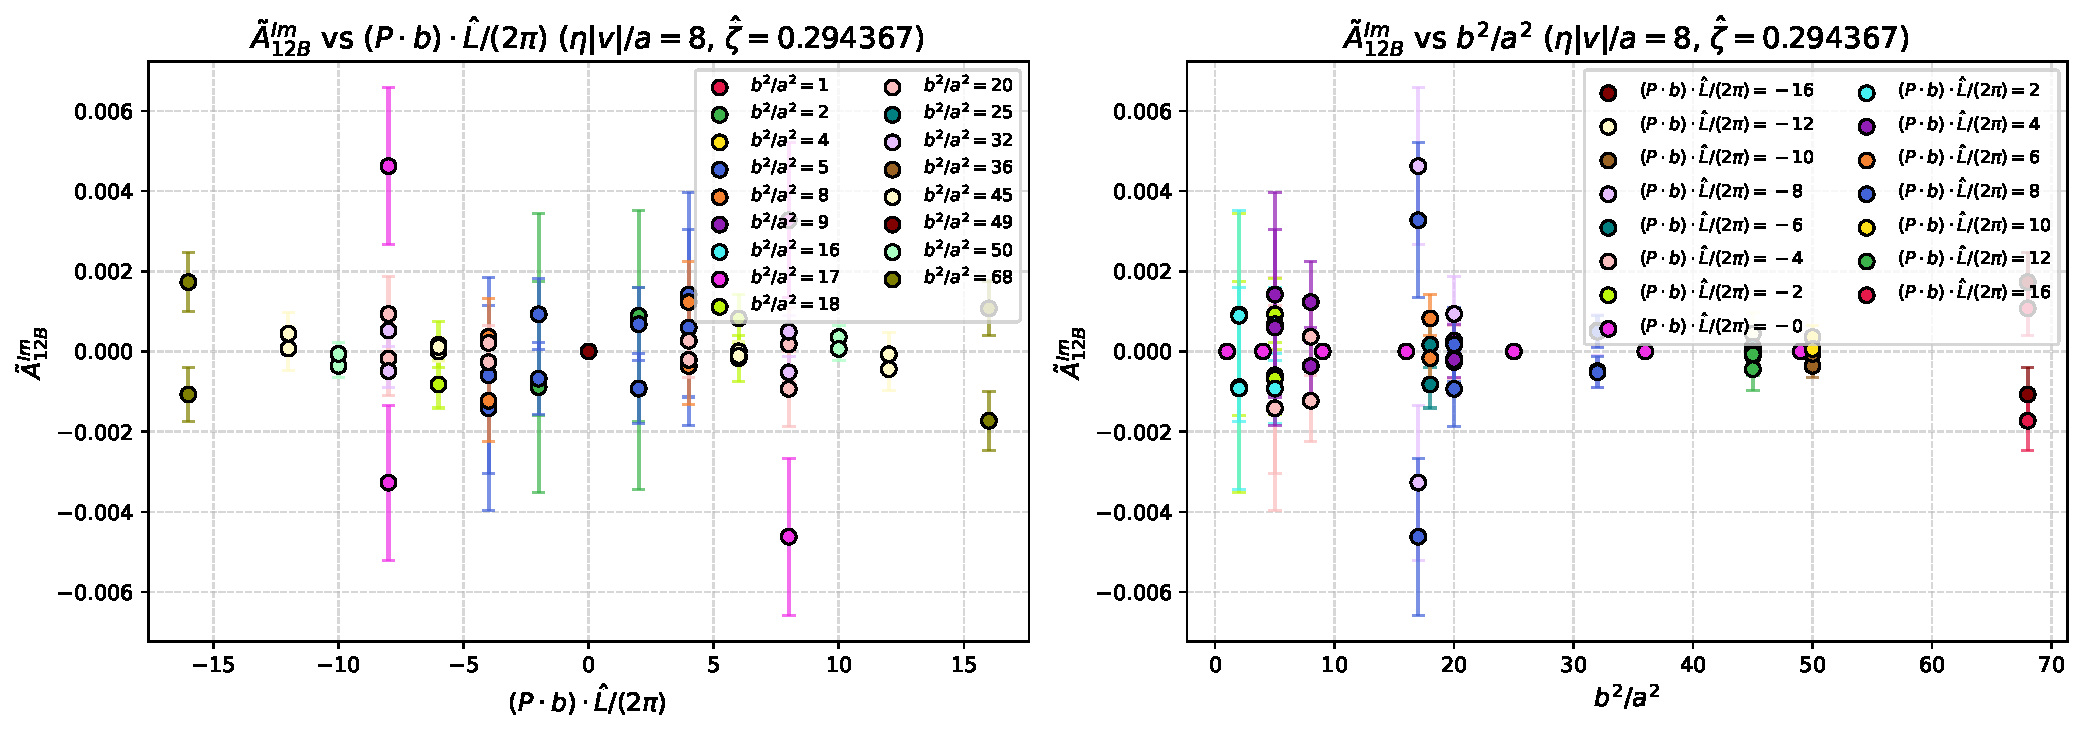
\includegraphics[width=0.48\linewidth]{figures/amps/ImA12B_Pb_bsq_eta8_PL-2_2D.pdf}
\caption{Real (left) and imaginary (right) parts of $\tAmp_{2B}$ (top) and $\tAmp_{12B}$ (bottom) in the $((\vect{P}\cdot\vect{b})\hat{L}/(2\pi),\,b^2/a^2)$ space at fixed $\eta|\vect{v}|/a=8$, for $\vect{P}\cdot a\hat{L}/(2\pi)=(-2,0,0)$ ($\hat\zeta=0.294367$).}
\label{fig:amps_P2}
\end{figure*}

\begin{figure*}[htbp]
\centering
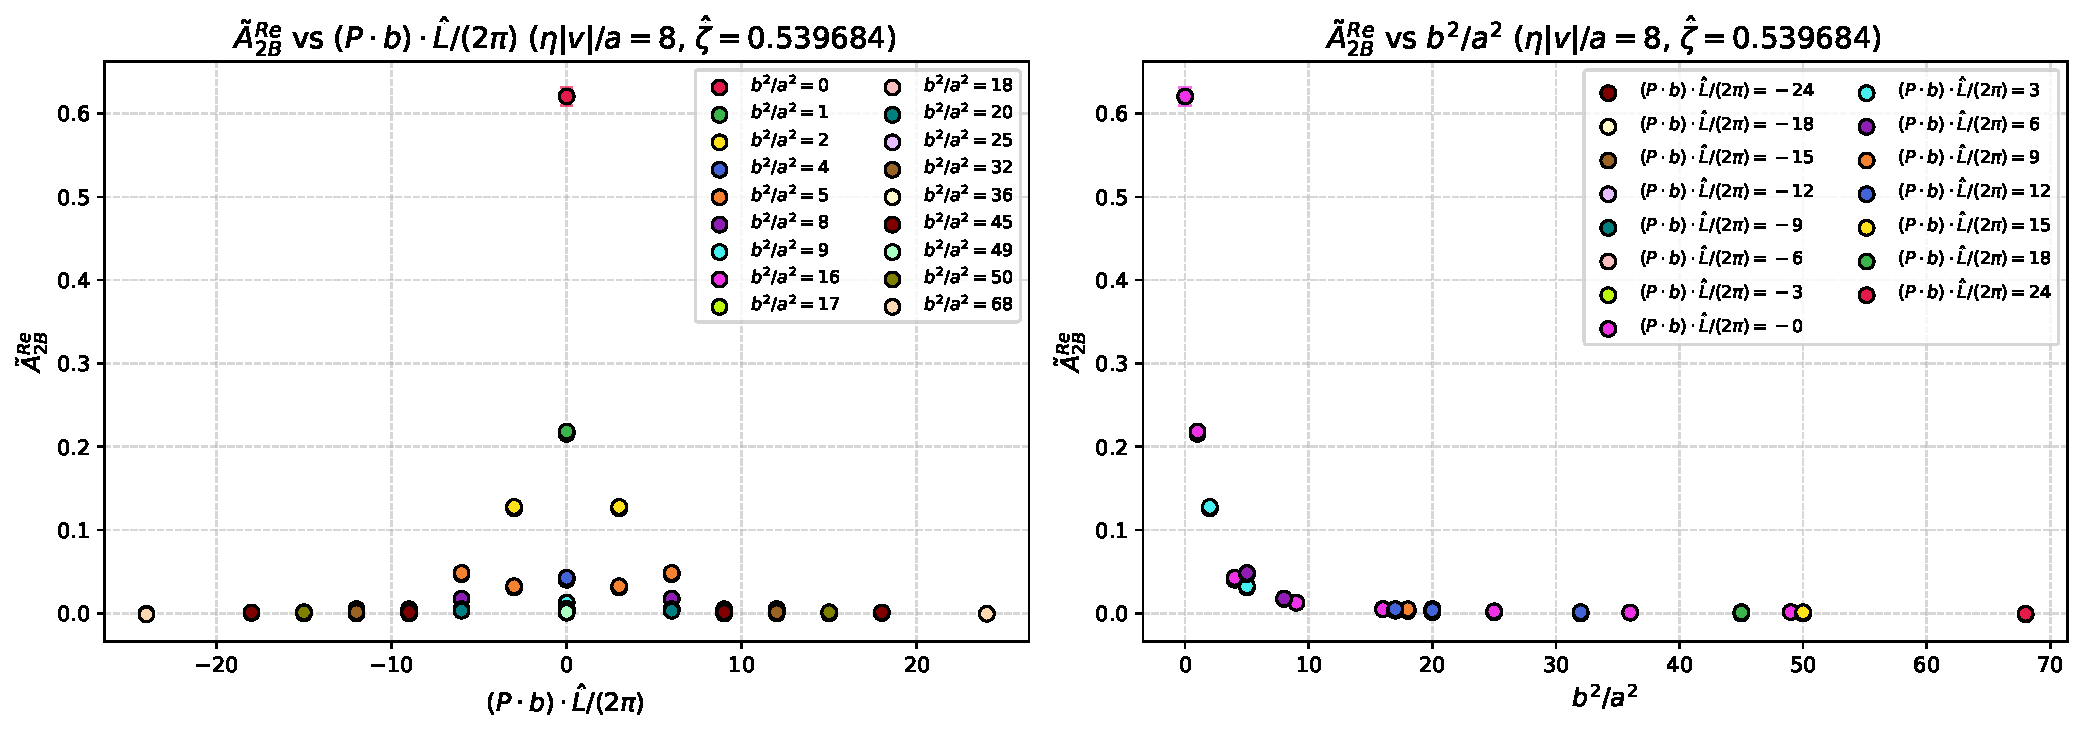
\includegraphics[width=0.48\linewidth]{figures/amps/ReA2B_Pb_bsq_eta8_PL-3_2D.pdf}\hfill
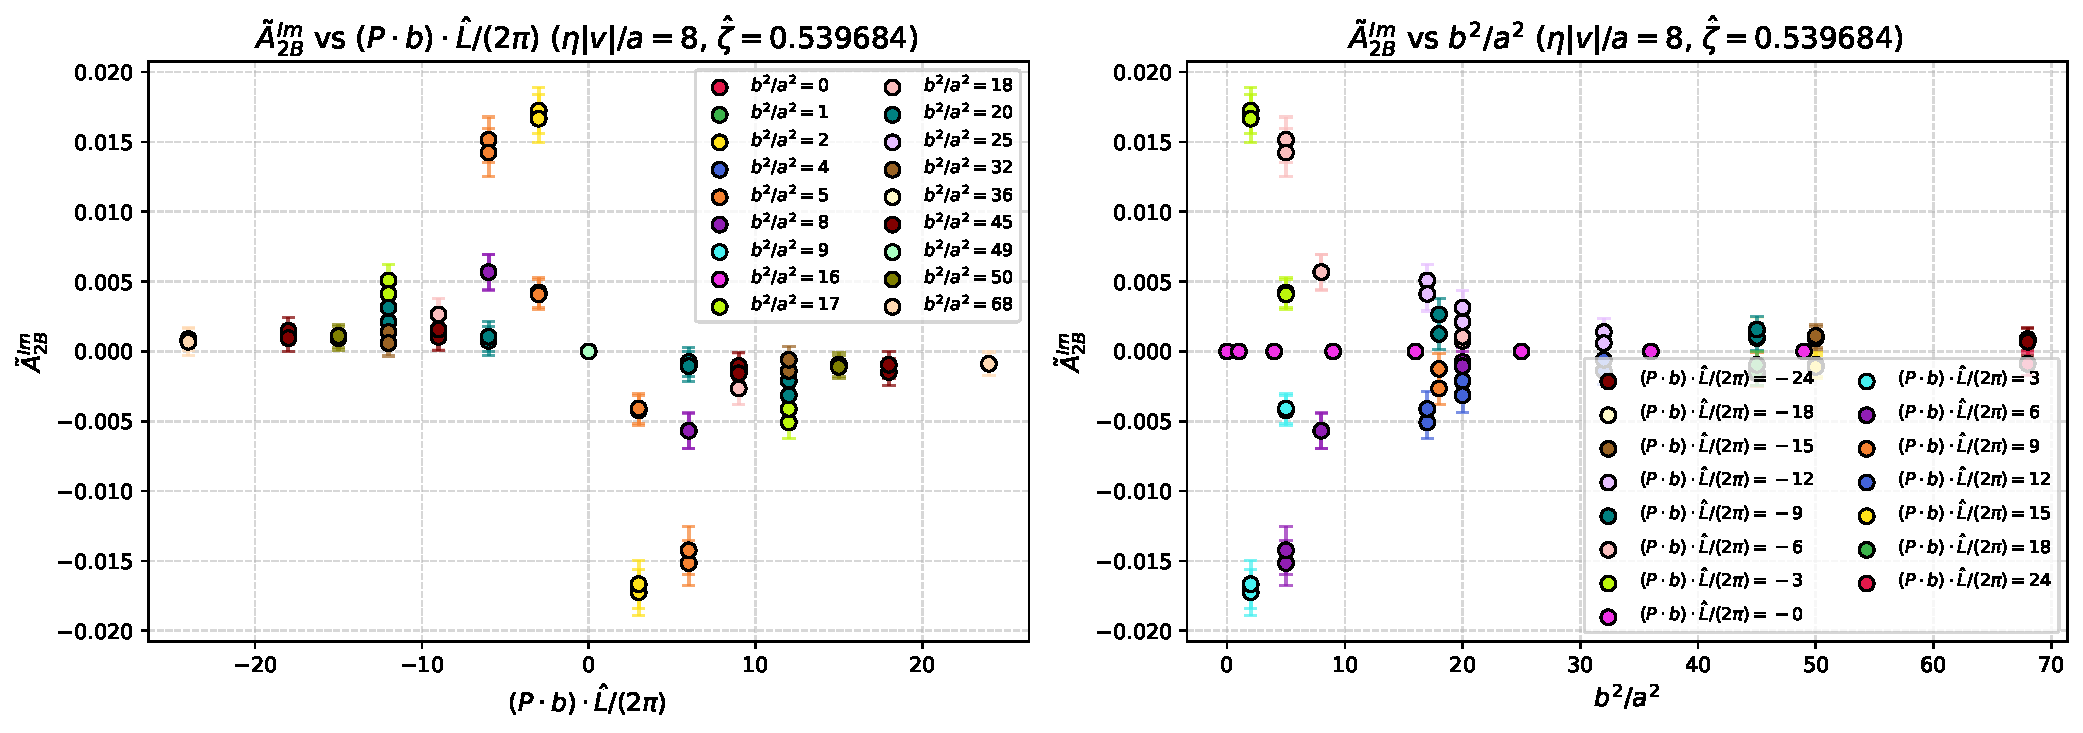
\includegraphics[width=0.48\linewidth]{figures/amps/ImA2B_Pb_bsq_eta8_PL-3_2D.pdf}\\[1ex]
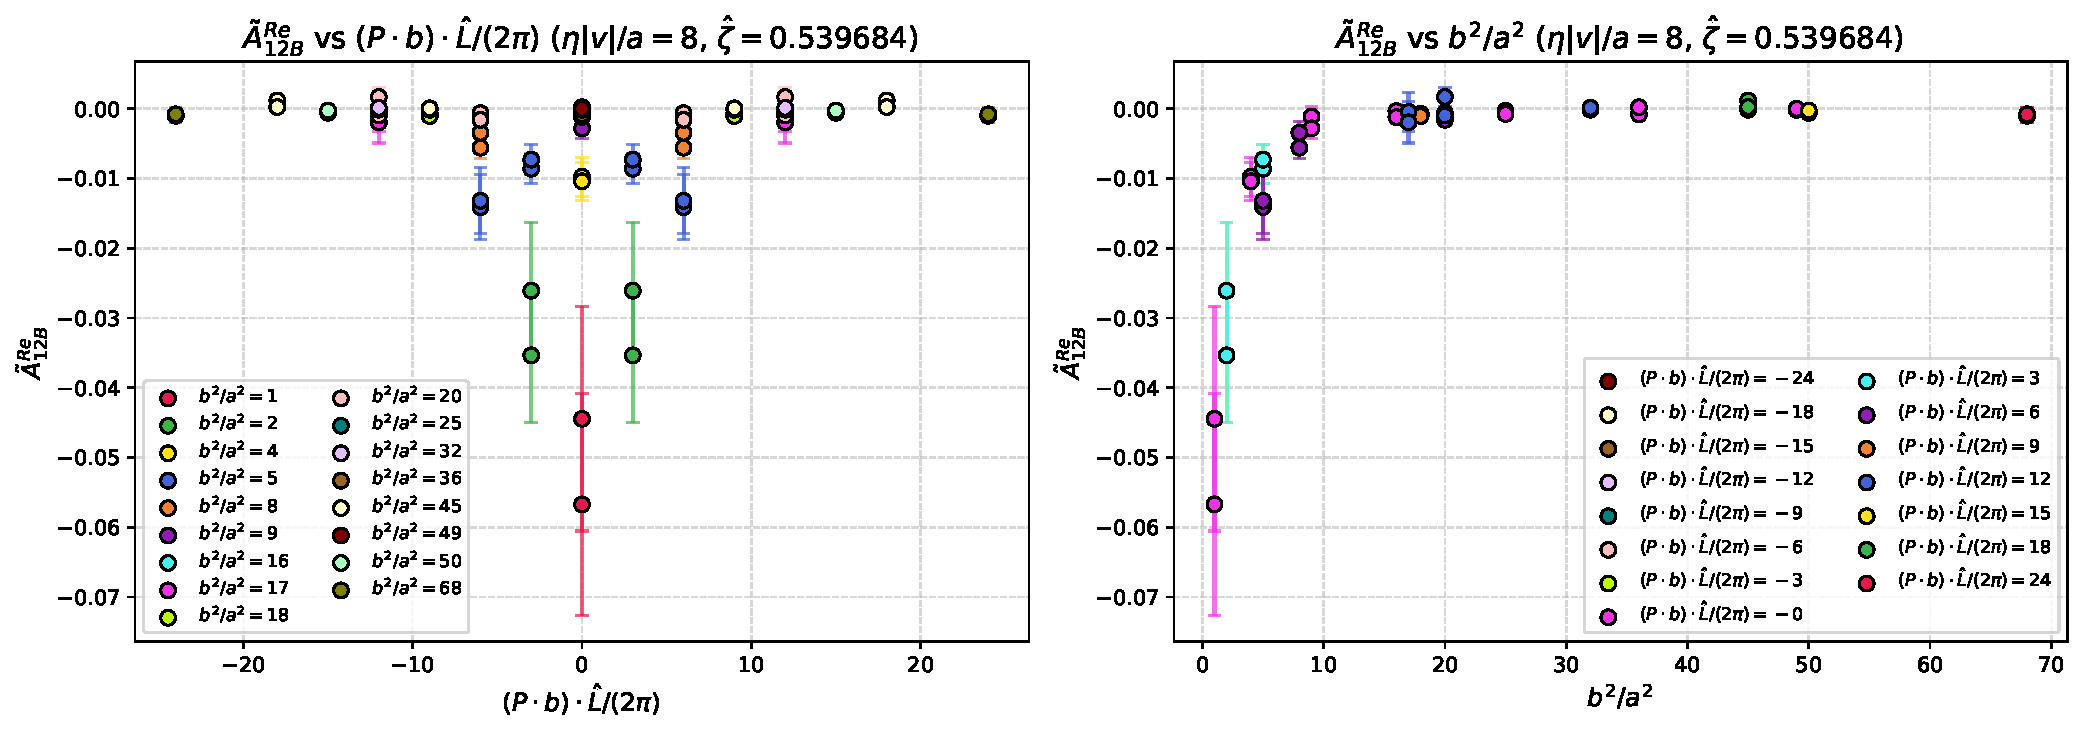
\includegraphics[width=0.48\linewidth]{figures/amps/ReA12B_Pb_bsq_eta8_PL-3_2D.pdf}\hfill
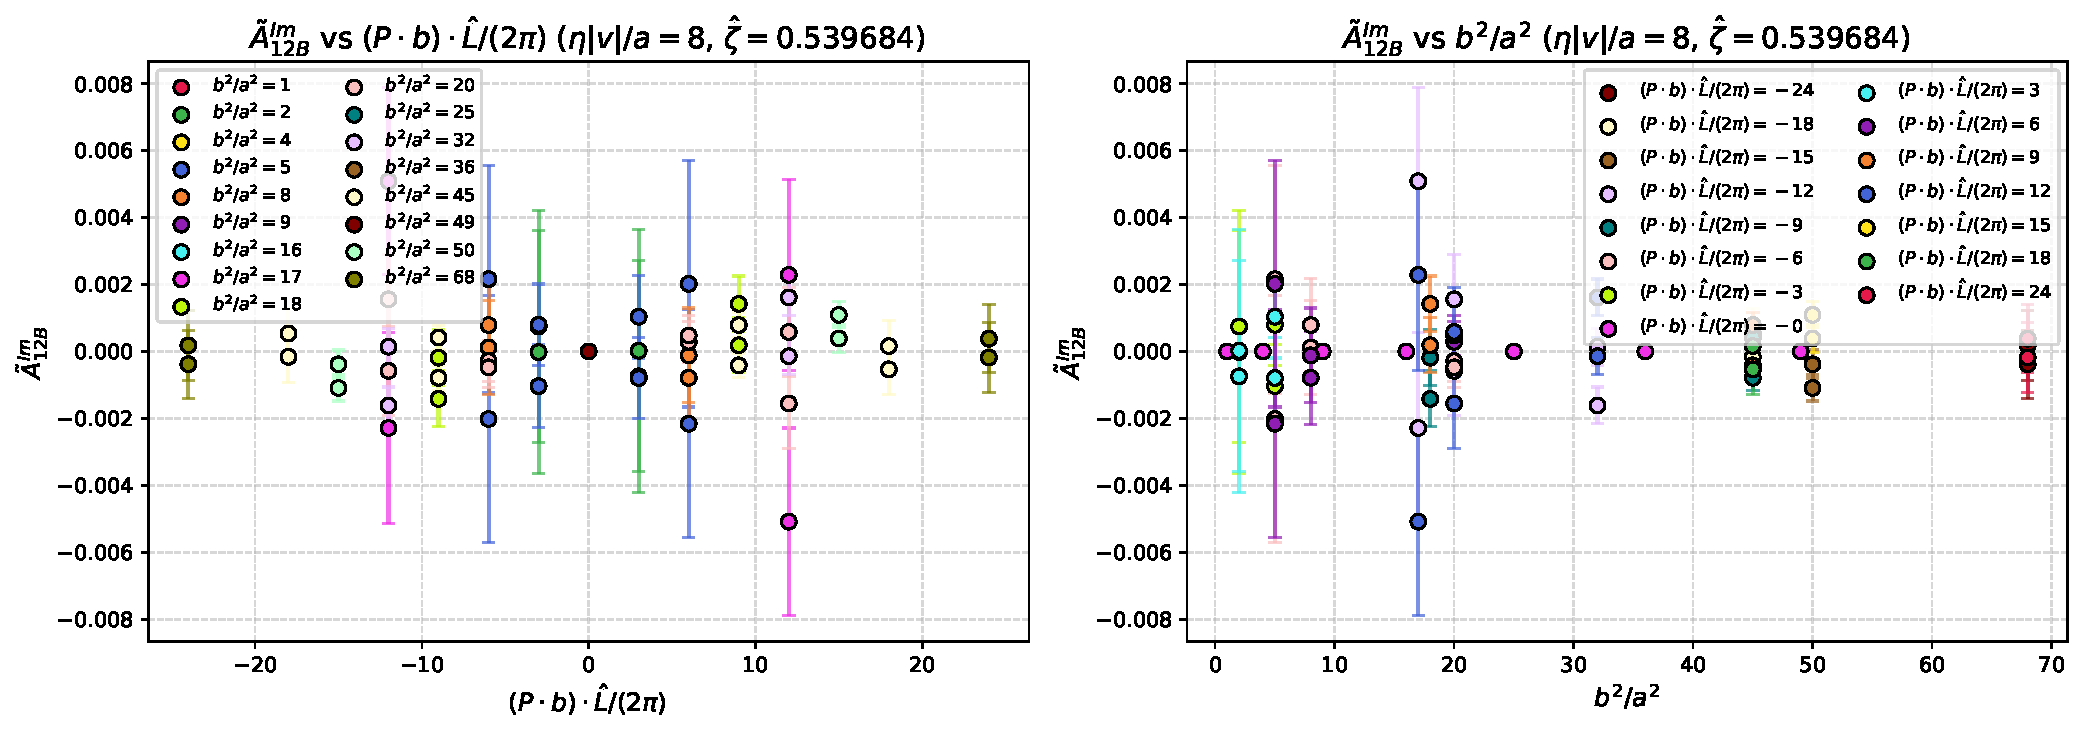
\includegraphics[width=0.48\linewidth]{figures/amps/ImA12B_Pb_bsq_eta8_PL-3_2D.pdf}
\caption{Real (left) and imaginary (right) parts of $\tAmp_{2B}$ (top) and $\tAmp_{12B}$ (bottom) in the $((\vect{P}\cdot\vect{b})\hat{L}/(2\pi),\,b^2/a^2)$ space at fixed $\eta|\vect{v}|/a=8$, for $\vect{P}\cdot a\hat{L}/(2\pi)=(-3,0,0)$ ($\hat\zeta=0.539684$).}
\label{fig:amps_P3}
\end{figure*}
